\documentclass[11pt,final,hidelinks]{article}
\usepackage[utf8]{inputenc}
\usepackage[T1]{fontenc}
\usepackage{lmodern}
\usepackage[margin=1in]{geometry}
\usepackage[english]{babel}
\usepackage{graphicx}
\usepackage[activate={true,nocompatibility},final,tracking=true,kerning=true,spacing=true,factor=1100,stretch=10,shrink=10]{microtype}
\usepackage{mathtools}
\usepackage{amsmath}
\usepackage{amsthm}
\usepackage{amssymb}
\usepackage{algorithm2e}
\usepackage{booktabs}
\usepackage{hyperref}
\usepackage[square,numbers]{natbib}
\bibliographystyle{plainnat}
\usepackage{cleveref}
\usepackage{tikz}
\usetikzlibrary{arrows.meta,positioning,shapes.geometric,calc,patterns}

% Theorem environments
\newtheorem{theorem}{Theorem}[section]
\newtheorem{lemma}[theorem]{Lemma}
\newtheorem{proposition}[theorem]{Proposition}
\newtheorem{corollary}[theorem]{Corollary}
\newtheorem{definition}[theorem]{Definition}
\newtheorem{example}[theorem]{Example}
\newtheorem{remark}[theorem]{Remark}
\newtheorem{construction}[theorem]{Construction}
\newtheorem{principle}[theorem]{Principle}

% Unified notation bridging both series
\newcommand{\Encode}[1]{\mathsf{encode}(#1)}
\newcommand{\ValidEnc}[1]{\mathsf{ValidEncodings}(#1)}
\newcommand{\Hash}[1]{h(#1)}
\newcommand{\Prob}[1]{\mathbb{P}[#1]}
\newcommand{\Card}[1]{|#1|}
\newcommand{\Bernoulli}[2]{\mathcal{B}^{#2}\langle #1 \rangle}
\newcommand{\Oblivious}[1]{\mathcal{O}\langle #1 \rangle}
\newcommand{\True}{\mathtt{true}}
\newcommand{\False}{\mathtt{false}}
\newcommand{\fprate}{\alpha}
\newcommand{\fnrate}{\beta}
\newcommand{\Uniform}[1]{\mathcal{U}(#1)}
\newcommand{\Freq}[1]{\mathsf{freq}(#1)}
\newcommand{\Leak}[1]{\mathcal{L}(#1)}

\title{Hash-Based Constructions: A Unified Framework for Bernoulli and Oblivious Types}
\author{
    Alexander Towell\\
    \texttt{atowell@siue.edu}
}
\date{\today}

\begin{document}
\maketitle

\begin{abstract}
We present a unified hash-based framework that underlies both Bernoulli types (probabilistic data structures with controlled error) and oblivious types (privacy-preserving computations with hidden access patterns). The key insight is that both paradigms can be constructed by finding seeds that map known inputs to valid output encodings, while unknown inputs naturally map randomly through the hash function. This framework reveals that Bloom filters, secure indexes, private information retrieval, and oblivious data structures are all instances of the same fundamental construction, differing only in how encoding sets are chosen. We show that error rates in Bernoulli types and privacy guarantees in oblivious types both emerge from the relative sizes of encoding sets. The framework provides a principled way to navigate trade-offs between space, accuracy, and privacy, while dramatically simplifying implementation through single hash evaluations rather than complex protocols.
\end{abstract}

\section{Introduction}

\subsection{Two Series, One Framework}

We have developed two series of papers:
\begin{enumerate}
    \item \textbf{Bernoulli Types}: Probabilistic data structures with controlled error rates
    \item \textbf{Oblivious Computing}: Privacy-preserving systems hiding access patterns
\end{enumerate}

This paper reveals they share a common foundation: hash-based constructions with encoding sets.

\subsection{The Unifying Insight}

Both paradigms follow the same construction pattern:
\begin{enumerate}
    \item Define encoding sets for each output value
    \item Find seeds mapping inputs to appropriate encodings
    \item Let unknown inputs map randomly via hash function
    \item Properties emerge from encoding set sizes
\end{enumerate}

The difference lies in the objective:
\begin{itemize}
    \item \textbf{Bernoulli}: Optimize for space with acceptable error
    \item \textbf{Oblivious}: Optimize for privacy with uniform distribution
\end{itemize}

\subsection{Moving Beyond Traditional Views}

\begin{center}
\begin{tabular}{lll}
\textbf{Structure} & \textbf{Traditional View} & \textbf{Unified View} \\
\hline
Bloom filter & Set bits with $k$ hashes & Map to True encoding \\
Secure index & Encrypt and store & Uniform encoding distribution \\
PIR & Complex protocols & Hierarchical encoding \\
ORAM & Tree-based shuffling & Oblivious encoding access \\
\end{tabular}
\end{center}

\section{The General Hash-Based Construction}

\subsection{Formal Framework}

\begin{definition}[Hash-Based Type Construction]
For function $f: X \to Y$, a hash-based construction consists of:
\begin{itemize}
    \item \textbf{Input encoding}: $\mathsf{encode}_X: X \to \{0,1\}^*$
    \item \textbf{Output encoding sets}: $\mathsf{encode}_Y: Y \to \mathcal{P}(\{0,1\}^m)$
    \item \textbf{Hash function}: $h: \{0,1\}^* \times \{0,1\}^s \to \{0,1\}^m$
    \item \textbf{Seed finding}: Algorithm to find $s$ such that:
    \begin{equation}
    \forall x \in X: \Prob{\Hash{\Encode{x} \| s} \in \ValidEnc{f(x)}} \geq 1 - \fnrate
    \end{equation}
\end{itemize}
\end{definition}

\subsection{Construction Algorithm}

\begin{algorithm}[H]
\caption{Universal Hash-Based Construction}
\KwIn{Function $f: X \to Y$, Objectives (space/privacy/accuracy)}
\KwOut{Seed $s$ and encoding sets achieving objectives}

\textbf{Step 1: Design encoding sets based on objective}\\
\eIf{Objective = Space-optimal Bernoulli}{
    $\Card{\ValidEnc{y}} \propto \Freq{y}$ \tcp{Entropy-optimal}
}{
\eIf{Objective = Privacy-optimal Oblivious}{
    $\Card{\ValidEnc{y}} \propto 1/\Freq{y}$ \tcp{Uniform output}
}{
    Choose custom encoding sizes\;
}}

\textbf{Step 2: Find suitable seed}\\
\Repeat{success}{
    $s \leftarrow$ random seed\;
    success $\leftarrow$ CheckSeed($f$, $s$, $\fnrate$)\;
}

\textbf{Step 3: Return implementation}\\
\Return{HashBasedType($s$, encoding sets)}
\end{algorithm}

\subsection{Key Properties}

\begin{theorem}[Emergent Properties from Encoding Sizes]
Given encoding sets with sizes $\Card{\ValidEnc{y}}$ for each $y \in Y$:
\begin{enumerate}
    \item \textbf{False positive rate}: $\fprate_y = \Card{\ValidEnc{y}}/2^m$
    \item \textbf{Output distribution}: $\Prob{\text{observe encoding } e} \propto \Freq{y}/\Card{\ValidEnc{y}}$
    \item \textbf{Information leakage}: $\Leak{} = \max_y \log(\Freq{y} \cdot 2^m / \Card{\ValidEnc{y}})$
\end{enumerate}
\end{theorem}

\section{The Spectrum of Encoding Strategies}

\subsection{Design Space}

\begin{figure}[h]
\centering
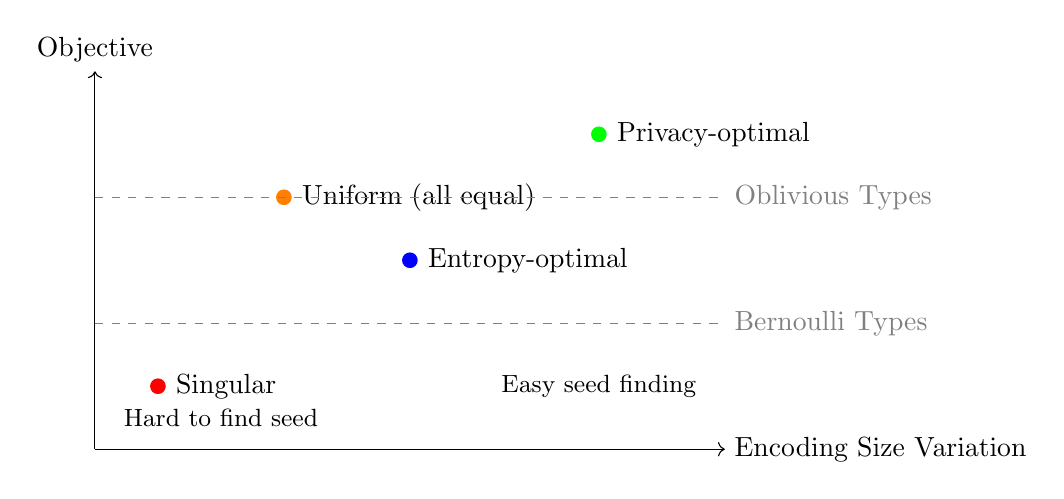
\begin{tikzpicture}[scale=0.8]
% Axes
\draw[->] (0,0) -- (10,0) node[right] {Encoding Size Variation};
\draw[->] (0,0) -- (0,6) node[above] {Objective};

% Points
\node[circle,fill=red,inner sep=2pt,label=right:{Singular}] at (1,1) {};
\node[circle,fill=blue,inner sep=2pt,label=right:{Entropy-optimal}] at (5,3) {};
\node[circle,fill=green,inner sep=2pt,label=right:{Privacy-optimal}] at (8,5) {};
\node[circle,fill=orange,inner sep=2pt,label=right:{Uniform (all equal)}] at (3,4) {};

% Regions
\draw[dashed,gray] (0,2) -- (10,2) node[right] {Bernoulli Types};
\draw[dashed,gray] (0,4) -- (10,4) node[right] {Oblivious Types};

% Annotations
\node[align=left] at (2,0.5) {\small Hard to find seed};
\node[align=left] at (8,1) {\small Easy seed finding};
\end{tikzpicture}
\caption{Spectrum of encoding strategies and their trade-offs}
\end{figure}

\subsection{Detailed Strategies}

\begin{center}
\begin{tabular}{llll}
\toprule
\textbf{Strategy} & \textbf{Encoding Rule} & \textbf{Properties} & \textbf{Use Case} \\
\midrule
Singular & $\Card{\ValidEnc{y}} = 1$ & Minimal space, hard seed & Theory only \\
Entropy & $\Card{\ValidEnc{y}} \propto \Freq{y}$ & Balanced, practical & Bloom filters \\
Privacy & $\Card{\ValidEnc{y}} \propto 1/\Freq{y}$ & Uniform output & Secure indexes \\
Uniform & $\Card{\ValidEnc{y}} = c$ & Simple, suboptimal & Basic systems \\
Custom & Application-specific & Flexible & Specialized \\
\bottomrule
\end{tabular}
\end{center}

\section{Bernoulli Types through Hash Construction}

\subsection{Bloom Filters Reimagined}

\begin{construction}[Hash-Based Bloom Filter]
For set $S \subseteq U$:
\begin{enumerate}
    \item Define $\ValidEnc{\True} = \{0, 1, \ldots, \lfloor\fprate \cdot 2^m\rfloor - 1\}$
    \item Find seed $s$ where $\forall x \in S: \Hash{\Encode{x} \| s} \in \ValidEnc{\True}$
    \item Membership test: Check if $\Hash{\Encode{x} \| s} \in \ValidEnc{\True}$
\end{enumerate}
Properties:
\begin{itemize}
    \item False positive rate: $\fprate$ (by design)
    \item False negative rate: 0 (by construction)
    \item Single hash evaluation (not $k$ hashes)
\end{itemize}
\end{construction}

\subsection{Bernoulli Maps}

\begin{construction}[Hash-Based Approximate Map]
For $f: X \to Y$:
\begin{enumerate}
    \item Partition $[0, 2^m)$ into regions for each $y \in Y$
    \item Region sizes determine error characteristics
    \item Find seed mapping most $x$ to correct regions
    \item Tolerate $\fnrate$ fraction mapping incorrectly
\end{enumerate}
\end{construction}

\begin{example}[Frequency Counter]
Count occurrences with controlled error:
\begin{itemize}
    \item Frequent values: Large encoding regions (accurate)
    \item Rare values: Small encoding regions (more error)
    \item Natural adaptation to data distribution
\end{itemize}
\end{example}

\section{Oblivious Types through Hash Construction}

\subsection{Achieving Perfect Obliviousness}

\begin{principle}[Uniformity Principle]
Perfect obliviousness achieved when:
\begin{equation}
\Card{\ValidEnc{y}} \cdot \Freq{y} = \text{constant}
\end{equation}
This ensures uniform distribution at observable layer.
\end{principle}

\begin{construction}[Oblivious Map via Uniform Encoding]
For $f: X \to Y$ with frequencies $\Freq{y}$:
\begin{enumerate}
    \item Set $\Card{\ValidEnc{y}} = C/\Freq{y}$ for constant $C$
    \item Find seed mapping inputs correctly
    \item Add noise queries with random inputs
    \item Result: Uniform observable behavior
\end{enumerate}
\end{construction}

\subsection{Noise Injection and Privacy}

\begin{theorem}[Natural Noise from Invalid Inputs]
For inputs $u \notin \{\Encode{x} : x \in X\}$:
\begin{itemize}
    \item $\Hash{u \| s}$ distributes uniformly over $\{0,1\}^m$
    \item No correlation with valid computations
    \item Provides perfect cover for real operations
\end{itemize}
\end{theorem}

\begin{remark}[Free Privacy]
Invalid inputs cost nothing to process but provide:
\begin{itemize}
    \item Frequency hiding
    \item Pattern obfuscation
    \item Plausible deniability
\end{itemize}
\end{remark}

\section{Composition and Complex Systems}

\subsection{Composing Hash-Based Types}

\begin{theorem}[Composition Properties]
For $f: X \to Y$ and $g: Y \to Z$ with seeds $s_f, s_g$:
\begin{enumerate}
    \item \textbf{Valid composition}: $(g \circ f)(x)$ computed correctly
    \item \textbf{Error accumulation}: $\fnrate_{g \circ f} \leq \fnrate_f + \fnrate_g - \fnrate_f \cdot \fnrate_g$
    \item \textbf{Noise propagation}: Invalid inputs remain random through composition
    \item \textbf{Privacy preservation}: Uniformity maintained if both maintain it
\end{enumerate}
\end{theorem}

\subsection{Building Complex Systems}

\begin{example}[Private Search Engine]
Combines multiple hash-based constructions:
\begin{verbatim}
class PrivateSearch:
    def __init__(self):
        # Bernoulli index for space efficiency
        self.index = HashBernoulliIndex(entropy_optimal=True)
        
        # Oblivious query processing for privacy
        self.query_proc = HashObliviousMap(uniform_output=True)
        
        # PIR for document retrieval
        self.doc_store = HashBasedPIR()
        
    def search(self, query):
        # Add noise queries
        self.inject_noise_queries()
        
        # Process with uniform distribution
        doc_ids = self.query_proc.process(query)
        
        # Retrieve documents obliviously
        return self.doc_store.retrieve(doc_ids)
\end{verbatim}
\end{example}

\section{Implementation Techniques}

\subsection{Seed Finding Strategies}

\begin{algorithm}[H]
\caption{Efficient Seed Finding}
\KwIn{Function $f$, encoding sets, max iterations}
\KwOut{Seed $s$ or failure}

\textbf{Strategy 1: Random Search}\\
\For{$i = 1$ to max\_iterations}{
    $s \leftarrow$ random()\;
    \If{CheckSeed($f$, $s$)}{
        \Return{$s$}\;
    }
}

\textbf{Strategy 2: Greedy Refinement}\\
$s \leftarrow$ random()\;
\While{not success and iterations $<$ max}{
    $s' \leftarrow$ Perturb($s$)\;
    \If{Score($s'$) $>$ Score($s$)}{
        $s \leftarrow s'$\;
    }
}

\textbf{Strategy 3: Solver-Based}\\
Encode as SAT/SMT problem\;
\Return{Solver.solve()}
\end{algorithm}

\subsection{Performance Optimizations}

\begin{enumerate}
    \item \textbf{Vectorization}: Process multiple hashes in parallel
    \item \textbf{Caching}: Store frequently accessed encodings
    \item \textbf{Lazy evaluation}: Compute encodings on demand
    \item \textbf{Hardware acceleration}: Use AES-NI for fast hashing
\end{enumerate}

\section{Analysis and Trade-offs}

\subsection{Space-Privacy-Accuracy Triangle}

\begin{theorem}[Fundamental Trade-off]
For hash-based construction with $m$-bit output:
\begin{equation}
\text{Space} \cdot \text{Privacy} \cdot \text{Accuracy} \leq 2^m
\end{equation}
Cannot simultaneously optimize all three.
\end{theorem}

\begin{proof}
\begin{itemize}
    \item Space requires small encodings: $\sum_y \Card{\ValidEnc{y}} \to \min$
    \item Privacy requires uniform output: $\Card{\ValidEnc{y}} \propto 1/\Freq{y}$
    \item Accuracy requires large encodings: $\Card{\ValidEnc{y}} \to \max$
\end{itemize}
These constraints conflict fundamentally.
\end{proof}

\subsection{Choosing the Right Point}

\begin{center}
\begin{tabular}{llll}
\toprule
\textbf{Application} & \textbf{Priority} & \textbf{Encoding Strategy} & \textbf{Trade-off} \\
\midrule
Caching & Space & Entropy-optimal & Accept false positives \\
Medical records & Privacy & Uniform output & Use more space \\
Network router & Accuracy & Large encodings & Sacrifice privacy \\
Encrypted DB & Balanced & Hybrid approach & Moderate all \\
\bottomrule
\end{tabular}
\end{center}

\section{Theoretical Implications}

\subsection{Unification of Disparate Fields}

This framework unifies:
\begin{itemize}
    \item \textbf{Probabilistic data structures}: Bloom filters, sketches, counters
    \item \textbf{Cryptographic protocols}: PIR, ORAM, secure indexes
    \item \textbf{Information theory}: Channel capacity, entropy coding
    \item \textbf{Privacy mechanisms}: Differential privacy, oblivious computing
\end{itemize}

All are instances of hash-based constructions with different encoding strategies.

\subsection{New Theoretical Questions}

\begin{enumerate}
    \item \textbf{Optimal encoding design}: Given constraints, find optimal encoding sizes
    \item \textbf{Seed complexity}: Characterize difficulty of seed finding
    \item \textbf{Composition theory}: How do properties compose through multiple layers?
    \item \textbf{Lower bounds}: What are fundamental limits of hash-based constructions?
\end{enumerate}

\section{Practical Applications}

\subsection{Simplified Implementations}

Traditional Bloom filter (complex):
\begin{verbatim}
class BloomFilter:
    def __init__(self, size, k_hashes):
        self.bits = BitArray(size)
        self.hashes = [HashFunction(i) for i in range(k_hashes)]
    
    def add(self, x):
        for h in self.hashes:
            self.bits[h(x) % size] = 1
            
    def contains(self, x):
        return all(self.bits[h(x) % size] for h in self.hashes)
\end{verbatim}

Hash-based construction (simple):
\begin{verbatim}
class HashBloomFilter:
    def __init__(self, items, fp_rate):
        self.threshold = int(fp_rate * 2**32)
        self.seed = self.find_seed(items)
    
    def contains(self, x):
        return hash(x + self.seed) < self.threshold
\end{verbatim}

\subsection{New Possibilities}

The framework enables:
\begin{itemize}
    \item \textbf{Adaptive structures}: Adjust encoding sizes dynamically
    \item \textbf{Hybrid systems}: Mix Bernoulli and oblivious properties
    \item \textbf{Cross-domain optimization}: Trade accuracy for privacy
    \item \textbf{Automatic synthesis}: Generate implementations from specifications
\end{itemize}

\section{Future Directions}

\subsection{Research Opportunities}

\begin{enumerate}
    \item \textbf{Automated encoding design}: ML-based optimization of encoding sizes
    \item \textbf{Quantum hash functions}: Post-quantum secure constructions
    \item \textbf{Differential privacy integration}: Combine with DP mechanisms
    \item \textbf{Hardware implementations}: Custom chips for hash-based types
\end{enumerate}

\subsection{Practical Developments}

\begin{enumerate}
    \item \textbf{Standard library}: Hash-based implementations of common structures
    \item \textbf{Compiler support}: Automatic conversion to hash-based types
    \item \textbf{Verification tools}: Prove properties of hash-based systems
    \item \textbf{Benchmarking suite}: Compare traditional vs hash-based
\end{enumerate}

\section{Related Work}

\subsection{Historical Context}

\begin{itemize}
    \item \textbf{1970}: Bloom introduces Bloom filters
    \item \textbf{1981}: Yao's garbled circuits for oblivious computing
    \item \textbf{1995}: Chor et al. introduce PIR
    \item \textbf{2000s}: Sketch data structures proliferate
    \item \textbf{2010s}: Practical oblivious computing systems
    \item \textbf{This work}: Unified hash-based framework
\end{itemize}

\subsection{Connections to Existing Theory}

\begin{itemize}
    \item \textbf{Learning theory}: Hash functions as random projections
    \item \textbf{Coding theory}: Encoding sets as error-correcting codes
    \item \textbf{Compressed sensing}: Sparse recovery through hashing
    \item \textbf{Locality-sensitive hashing}: Similar encoding principles
\end{itemize}

\section{Conclusions}

\subsection{Key Contributions}

We have shown that:
\begin{enumerate}
    \item \textbf{Unification}: Bernoulli and oblivious types share hash-based foundation
    \item \textbf{Simplification}: Single hash evaluation replaces complex protocols
    \item \textbf{Emergence}: Properties emerge from encoding set sizes
    \item \textbf{Composition}: Natural framework for building complex systems
\end{enumerate}

\subsection{Paradigm Shift}

This represents a fundamental shift in thinking:

\begin{center}
\begin{tabular}{ll}
\textbf{Old View} & \textbf{New View} \\
\hline
Design data structures & Design encoding sets \\
Implement protocols & Find seeds \\
Add noise explicitly & Leverage natural randomness \\
Analyze each separately & Unified analysis framework \\
\end{tabular}
\end{center}

\subsection{Final Thoughts}

The hash-based construction framework reveals deep connections between seemingly disparate fields. By understanding that both probabilistic data structures and privacy-preserving systems are managing the same fundamental challenge—controlling what happens to known inputs while accepting randomness for unknown inputs—we gain powerful new tools for system design.

The elegance of this approach lies not in its complexity but in its simplicity: 
\begin{itemize}
    \item One hash function
    \item One seed-finding algorithm
    \item Encoding sets sized for objectives
    \item Natural randomness for everything else
\end{itemize}

This simplicity, combined with the framework's generality, suggests it should be the default approach for implementing both Bernoulli and oblivious types.

\bibliography{references}

\appendix

\section{Quick Reference}

\subsection{Encoding Size Formulas}

\begin{center}
\begin{tabular}{ll}
\textbf{Objective} & \textbf{Encoding Size Rule} \\
\hline
Minimize space & $\Card{\ValidEnc{y}} = \fprate \cdot 2^m$ \\
Maximize privacy & $\Card{\ValidEnc{y}} = C/\Freq{y}$ \\
Entropy-optimal & $\Card{\ValidEnc{y}} = 2^{m \cdot H(y)/H_{max}}$ \\
Fixed error rate & $\Card{\ValidEnc{y}} = \fprate_y \cdot 2^m$ \\
\end{tabular}
\end{center}

\subsection{Common Patterns}

\begin{verbatim}
# Pattern 1: Bernoulli Set
ValidEnc[True] = [0, α*2^m)
ValidEnc[False] = [α*2^m, 2^m)

# Pattern 2: Oblivious Map
for y in Y:
    ValidEnc[y] = [start[y], start[y] + size[y])
    where size[y] * freq[y] = constant

# Pattern 3: Approximate Counter
ValidEnc[count] = [count*scale - ε, count*scale + ε]
\end{verbatim}

\end{document}